\chapter{区域积分}
\label{chap:region-integrals}
\label{chap:multivariate-integration}

一元积分沿区间累计：把区间切成小段，每段的长度乘函数值再相加。许多总量却分布在平面或空间的一块区域上，例如薄板的质量、物体的体积、一个地区的平均降雨量。本章要回答：怎样的区域有确定的体积，怎样的函数可以在区域上累计；累计出的数怎样实际算出来；换坐标或让被积函数带参数时，哪些操作是合法的。

第一节仿照一元Riemann积分，用坐标盒从内外两侧逼近区域，得到Jordan区域和它的体积，再用分割和定义积分，并整理线性、保序与区域可加性。定义同时分割全部坐标，不便直接计算，所以第二节在连续性条件下把多维积分化为逐坐标的一元积分；上下限由区域的截面决定，换序时要重新描述区域。无界区域或无界函数则要先截断，不同的截断方式可能给出不同的结果。

第三节用坐标变换简化区域。参数空间中同样大小的小块，映到原空间后体积不同，Jacobian行列式的绝对值给出这一局部倍数；变换还必须单次覆盖区域，奇异坐标点要先截去再取极限。第四节研究依赖参数的积分，说明在什么统一控制下可以对参数取极限、在积分号下求导，以及积分限随参数移动时怎样计入边界贡献。

本章使用第~\ref{chap:multivariate-differentiation}章的Jacobian、链式法则与连续偏导数判据，第~\ref{chap:normed-inner-product-spaces}章闭有界集上连续函数的一致连续性，以及一元Riemann积分和微积分基本定理，可参考\BookChapterRef{chap:univariate-integration}{卷一“一元函数的积分”章}。所建立的区域积分是后面路径积分、曲面积分和积分定理的共同基础。

\section{区域积分的定义与性质}
\label{sec:multivariable-region-integration}

一块不均匀的金属薄片占据平面区域$D$，在点$(x,y)$附近每单位面积的质量为$\rho(x,y)$。
把$D$切成许多小块，每块的质量约等于块内某一点的密度乘这块的面积。把各块的质量相加，就得到总质量的近似值；小块切得越细，近似越准确。
空间物体的质量、带电体的总电荷也这样累计，只是面积换成体积，面密度换成体密度或电荷密度。
这类问题中的被积函数都是多元标量函数$f:D\subseteq\mathbb R^d\to\mathbb R$。它的输入是一个位置的$d$个坐标，输出是该位置上待累计的一个数。

同一个积分还有两种常用读法。
若$f\geq0$定义在平面区域$D$上，积分等于以$D$为底、以$f$的图像为顶的立体的体积。这是一元积分“曲线下方的面积”在高一维的对应。
当$D$的面积有限且非零时，积分除以面积就是$f$在$D$上的平均值，例如一个地区的平均降雨量或一块薄板的平均温度。

本节把一元Riemann积分推广到有界区域上。先说明怎样的区域有确定的体积，再用分割和定义积分，最后整理积分的基本性质。一般可测函数与积分的极限定理在卷四中建立，本章不以它们为前提，可参考\BookChapterRef{chap:integration}{卷四“积分”章}。

\subsection{盒体积与Jordan可测性}

一元积分把区间切成小区间，每个小区间的长度都已知。多元积分要把区域切成小块，首先需要知道小块的体积。最简单的小块是坐标盒。
闭坐标盒$Q=\prod_{j=1}^d[a_j,b_j]$的体积定义为
\[
 \operatorname{vol}(Q)=\prod_{j=1}^d(b_j-a_j).
\]
某条边长度为零时，体积为零。

盒体积满足有限可加性。沿某个坐标把盒切成两块，被切的边长相加仍等于原边长，所以两块体积之和等于原体积。反复这样切，可知任意有限网格中小盒的体积之和都等于原盒体积。相邻小盒只共享边界，公共边界不重复贡献体积。

一般区域不是盒，它的体积用盒从内外两侧逼近。
设$D\subset\mathbb R^d$有界。取有限个内部互不相交、且都含于$D$的盒，它们的总体积从内侧估计$D$的体积；再取有限个内部互不相交、并合起来覆盖$D$的盒，它们的总体积从外侧估计。
若对每个$\varepsilon>0$，都能选出这样的内侧盒组和外侧盒组，使两者总体积之差小于$\varepsilon$，就称$D$为\term{Jordan可测}集合，简称Jordan区域。

任何一组内侧盒的总体积都不超过任何一组外侧盒的总体积；两侧差距又可以任意小，所以夹在两侧之间的数只有一个。这个数称为$D$的Jordan体积，记为$|D|$。它不依赖所选的盒组。

按定义检查内外逼近并不方便。下面的判别把问题归结为边界：有界集合$D$是Jordan可测的，当且仅当它的边界$\partial D$能被有限个总体积任意小的盒覆盖。

先证明充分性，关键是下面的观察。不在边界上的点，要么有一个邻域完全落在$D$内，要么有一个邻域完全落在$D$外。所以一个小盒若同时含有$D$的点和$D$外的点，它必与边界相交。

设边界可被总体积小于$\varepsilon/2$的有限个盒覆盖。把这些盒的各边稍微向外扩张，使总体积仍小于$\varepsilon$。盒的个数有限，所以可以在一个包含$D$的盒上取足够细的网格，使每个与边界相交的网格小盒都落入某个扩张盒。网格小盒内部互不重叠，因此与边界相交的小盒总体积小于$\varepsilon$。

取含于$D$的网格小盒作内侧逼近，取与$D$相交的网格小盒作外侧逼近。两者之差只由同时接触$D$和$D$外的小盒组成，这些小盒都与边界相交，总体积小于$\varepsilon$。所以$D$是Jordan可测的。

反过来，设$D$是Jordan可测的。边界上的点不在内侧盒组的内部，却在外侧盒组之中，所以边界含于“外侧盒组减去内侧盒组内部”所剩的部分。这部分的体积不超过两侧总体积之差，另外至多含有有限个盒的边界。盒的边界同样可以用总体积任意小的有限个盒覆盖，所以整个边界也可以。

这一判别也说明边界为何不影响累计。只要被积函数有界，落在边界附近的小块的总贡献，就不超过函数绝对值的上界乘覆盖盒的总体积，可以任意小。

例如闭圆盘是Jordan可测的。把圆周分成有限条足够短的弧，每条弧用一个小正方形覆盖。弧长尺度缩小时，所需正方形的个数按尺度的倒数增长，每个正方形的面积按尺度的平方缩小，所以总面积趋于零。
同样，有限条分段光滑曲线围成的平面区域，以及有限片光滑曲面围成的有界立体，其边界都能这样覆盖。这里依赖于边界只有有限片，且每片有足够规则的参数化；不能仅凭边界“看起来像曲线或曲面”就忽略它。

\subsection{多元Riemann和与可积性}

有了Jordan区域，就可以仿照一元情形定义积分。先在坐标盒上定义，再推广到一般区域。

设$R$是包含$D$的闭坐标盒。沿各坐标作有限分割，得到小盒$Q_1,\ldots,Q_N$，各小盒直径的最大值称为网格大小。在每个$Q_i$中任选取样点$\bm\xi_i$，对$R$上的有界函数$g$作Riemann和
\[
 S(g,P,\bm\xi)=\sum_{i=1}^N g(\bm\xi_i)\operatorname{vol}(Q_i).
\]
若网格大小趋于零时，无论怎样选取分割和取样点，这些和都趋于同一个有限值，就称$g$在$R$上Riemann可积，这个极限记作$\int_R g(\bm x)\,\mathrm d\bm x$。
这一要求针对所有足够细的分割和所有取样方式，而不只是某一种选点方式。

逐一检查所有取样方式并不可行，常用上和与下和来判断。
在每个小盒上分别取$g$的上确界和下确界，乘盒体积再求和，得到上和$U(g,P)$与下和$L(g,P)$。任意取样所得的Riemann和都夹在二者之间。因此，$g$可积当且仅当分割足够细时$U(g,P)-L(g,P)$可以任意小。

连续函数满足这一条件。若$g$在$R$上连续，由于$R$是紧集，$g$一致连续。网格足够细时，每个小盒上函数的最大值与最小值相差任意小；上和与下和之差不超过这个差值乘$R$的体积，因而任意小。所以$g$可积。

一般区域上的积分通过零延拓化为盒上的积分。
设$D$是有界Jordan区域，$f$是$D$上的有界函数。令$g=f\mathbb I_D$，即$g$在$D$上等于$f$，在$R\setminus D$上取零。若$g$在$R$上Riemann可积，就把它的积分定义为$\int_D f$。换一个更大的包含盒，只是多了一片取零的区域，积分不变。

若$f$能连续延拓到闭包$\overline D$，则零延拓可积。延拓后的函数在闭包上一致连续，所以远离边界的小盒上，函数的振幅可以任意小；靠近边界的小盒，由前面的边界覆盖控制总体积。两部分对上下和之差的贡献都可以任意小。
同样的论证适用于分块连续的有界函数：区域分成有限块，函数在每块上连续，不连续点只落在各块的边界上。函数在这些边界上怎样取值，不影响积分。

连续是可积的充分条件，但不是必要条件。例如在$R=[0,1]^2$上令$g(x,y)=\mathbb I_{\{x\geq1/2\}}$。它在直线$x=1/2$上不连续，但只有穿过这条直线的网格小盒会让上和与下和不同。这些小盒的总面积随网格变细而趋于零，所以$g$可积，积分为$1/2$。

另一方面，函数有界并不足以保证可积。$\mathbb I_{\mathbb Q^2}$在每个非退化小盒内既取$0$也取$1$，上和与下和之差始终等于$R$的面积，所以它不可积。

\subsection{积分的基本性质}

区域积分的基本性质都由有限Riemann和的相应性质取极限得到。积分是线性的。积分保持大小关系：若$f$、$h$可积且$f\leq h$，则
\[
 \int_D f\leq\int_D h.
\]
积分还满足绝对值估计$\bigl|\int_D f\bigr|\leq\int_D|f|$。
若有限个Jordan区域内部互不重叠，只沿可忽略的公共边界拼接，则在拼成的区域上的积分等于各块上的积分之和，这就是区域可加性。

常见的累计量都可以写成区域积分。取$f=1$得到体积$|D|$；非负密度$\rho$的积分是总质量$M=\int_D\rho$。当$|D|>0$时，$f$的平均值为
\[
 \frac1{|D|}\int_D f.
\]
当$M$有限且非零时，质心为
\[
 \frac1M\int_D\bm x\,\rho(\bm x)\,\mathrm d\bm x,
\]
其中向量值函数的积分按分量计算。

\section{累次积分}

区域积分的定义同时分割所有坐标。实际计算时，我们希望先沿一个坐标方向积分，再沿其余方向积分，把一次$d$维累计化为几次一元积分。本节说明这在什么条件下成立，以及上下限怎样由区域的截面确定。

\subsection{长方体上的累次积分}

先看矩形。设$f$在闭矩形$R=[a,b]\times[c,d]$上连续。固定$x$时，$y\mapsto f(x,y)$连续，所以一元积分
\[
 F(x)=\int_c^d f(x,y)\,\mathrm dy
\]
存在。$f$在$R$上一致连续，所以$x$的变化足够小时，所有$y\in[c,d]$处的函数值同时变化很小，$F$因而连续。

取乘积网格，把Riemann和中的项按列分组。每一列的内层求和趋于该列上$y$方向的积分，一致连续性保证所有列的误差同时很小；外层求和再趋于$\int_a^bF(x)\,\mathrm dx$。按行分组同理，于是
\[
 \int_R f(x,y)\,\mathrm d(x,y)
 =\int_a^b\left(\int_c^d f(x,y)\,\mathrm dy\right)\mathrm dx
 =\int_c^d\left(\int_a^b f(x,y)\,\mathrm dx\right)\mathrm dy.
\]
更多坐标的闭盒可以重复这样分组。

连续性是便于核对的充分条件。对一般的Riemann可积函数，某些截面上的一元积分可能不存在，所以不能只因整体可积就省去对内层积分的检查。

\subsection{简单区域上的累次积分}

一般区域上，累次积分的上下限由截面决定。设
\[
 D=\{(x,y):a\leq x\leq b,\ \alpha(x)\leq y\leq\beta(x)\},
\]
其中边界函数$\alpha\leq\beta$连续，且$f$在$D$的闭包上连续，则
\begin{equation}
 \int_D f(x,y)\,\mathrm d(x,y)
 =\int_a^b\left(\int_{\alpha(x)}^{\beta(x)}f(x,y)\,\mathrm dy\right)\mathrm dx.
\label{eq:classical-iterated-integral-simple-region}
\end{equation}
这同样是对零延拓的网格分组。边界曲线附近的格子总体积可以任意小，其余格子按截面累计。边界函数连续，在紧区间上一致连续，所以截面的端点随$x$一致变化，内层积分也随$x$连续。
由有限个这样的区域拼成的区域可以逐块计算，公共边界不重复累计。

换一种积分次序时，要重新求出区域在另一坐标轴上的投影和相应的截面。例如取$D=\{0\leq y\leq x\leq1\}$和$f(x,y)=x+y$。固定$x$，截面为$0\leq y\leq x$，得到
\[
 \int_0^1\left(\int_0^x(x+y)\,\mathrm dy\right)\mathrm dx
 =\int_0^1\frac{3x^2}{2}\,\mathrm dx=\frac12.
\]
固定$y$，截面变为$y\leq x\leq1$，同一个积分也等于
\[
 \int_0^1\left(\int_y^1(x+y)\,\mathrm dx\right)\mathrm dy
 =\int_0^1\left(\frac12+y-\frac{3y^2}{2}\right)\mathrm dy=\frac12.
\]
两组上下限描述的是同一个三角形的两种截面，而不是把积分号机械地交换。


图~\ref{fig:v2-integration-slices}在同一三角形中分别画出竖截面和横截面。先确定截面的两个端点，再写内层积分的上下限，便不会把换序误当成仅交换两个积分号。
\begin{figure}[!htb]
\centering
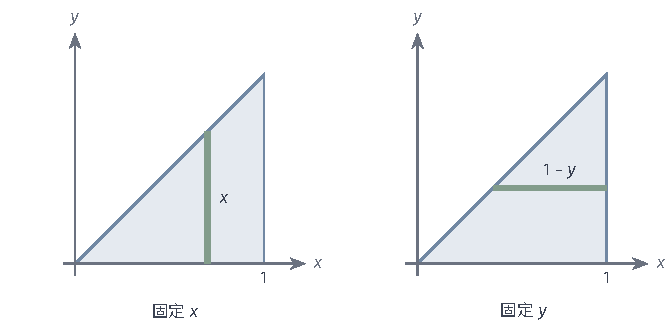
\includegraphics[width=112mm]{figures/02-vectors-matrices-and-multivariate-calculus/04-multivariate-calculus/tikz/explanation-additions/integration-slices.pdf}
\caption{区域$D=\{0\leq y\leq x\leq1\}$的两种切片。左图固定$x$，绿色线段从$y=0$到$y=x$；右图固定$y$，绿色线段从$x=y$到$x=1$。两种积分次序覆盖同一片区域。}
\label{fig:v2-integration-slices}
\end{figure}

换序还可能改变分块方式。考虑下面的三角形区域：
\[
 0\leq x\leq2,\qquad 0\leq y\leq\min(x,2-x).
\]
先对$y$积分时，上限在$x=1$处改变公式，需要分成两块。

先对$x$积分时，截面是$y\leq x\leq2-y$，$y$取遍$[0,1]$，一块即可。取$f=1$核对，两种次序都给出面积$1$。

\subsection{反常重积分与积分次序}

前面的结论只针对有界区域上的有界函数。区域无界，或被积函数在某点附近无界时，Riemann和不能直接使用。常用的做法是截断：选一族有界Jordan区域$D_\varepsilon$，它们避开奇点或截去远处，先逐个检查$f$在每个$D_\varepsilon$上Riemann可积，再考察$\int_{D_\varepsilon}f$的极限。
需要注意，沿某一族截断得到的极限，不能说明其他截断方式会给出同一结果。

例如在$(0,1]^2$上取
\[
 f(x,y)=\frac{x^2-y^2}{(x^2+y^2)^2}.
\]
对$0<\varepsilon<1$，先用矩形$D_\varepsilon=[\varepsilon,1]\times[\varepsilon^2,1]$截断。每个截断矩形都远离原点，$f$在其上连续。

先把下边界暂时放宽到$y=0$。对固定的$x>0$，$y\mapsto f(x,y)$在$[0,1]$上连续，原函数为$y/(x^2+y^2)$，所以
\[
 \int_\varepsilon^1\left(\int_0^1 f(x,y)\,\mathrm dy\right)\mathrm dx
 =\int_\varepsilon^1\frac{\mathrm dx}{1+x^2}
 \longrightarrow\frac\pi4.
\]
放宽时多算的窄条是$[\varepsilon,1]\times[0,\varepsilon^2]$。由$|x^2-y^2|\leq x^2+y^2$，窄条上
\[
 |f(x,y)|\leq\frac1{x^2+y^2}\leq\frac1{x^2},
\]
所以它的贡献不超过
\[
 \varepsilon^2\int_\varepsilon^1x^{-2}\,\mathrm dx\longrightarrow0.
\]
因此$\int_{D_\varepsilon}f\to\pi/4$。

交换两条边的截断速度，改用$E_\varepsilon=[\varepsilon^2,1]\times[\varepsilon,1]$。由$f(y,x)=-f(x,y)$，所得极限是$-\pi/4$。
两族矩形都逐渐填满同一个区域$(0,1]^2$，极限却不同，所以这里没有与截断方式无关的总量。
同样的计算也说明累次积分不能随意换序：两种次序的累次积分分别为
\[
 \int_0^1\left(\int_0^1f\,\mathrm dy\right)\mathrm dx=\frac\pi4,\qquad
 \int_0^1\left(\int_0^1f\,\mathrm dx\right)\mathrm dy=-\frac\pi4 .
\]

\section{区域积分的换元}
\label{sec:classical-change-variables}

圆盘用半径和角度描述，比用两个直角坐标简单。但换坐标不只是替换函数中的变量：参数空间中大小相同的小块，映到原空间后体积可能不同。线性映射把体积乘以其行列式的绝对值；可微映射在足够小的范围内近似线性。换元公式就是把这些局部的体积比例累计起来。

\subsection{积分换元公式}

为了保证每个点只被计算一次，并便于处理边界，先在两个开集之间取一个可微双射，再在其中选取有界的积分区域。
\begin{theorem}[经典区域积分的换元]
\label{thm:classical-change-of-variables}
设$U,V\subseteq\mathbb R^d$为开集，$T:U\to V$为$C^1$双射，逆映射也为$C^1$。设$E\subset U$为紧Jordan区域，且$T(E)$也是Jordan区域。若$f$在$T(E)$上连续，则
\begin{equation}
 \int_{T(E)}f(\bm x)\,\mathrm d\bm x
 =\int_E f(T(\bm u))|\det DT(\bm u)|\,\mathrm d\bm u.
\label{eq:classical-change-of-variables}
\end{equation}
\end{theorem}

下面说明权重$|\det DT|$的来源，并概述证明的思路。
取$E$附近的等边网格。对其中的小立方体，连续可微性给出一阶近似
\[
 T(\bm u+\bm h)-T(\bm u)=DT(\bm u)\bm h+\bm R_{\bm u}(\bm h).
\]
当$\|\bm h\|\leq\delta$时，余项满足
\[
 \|\bm R_{\bm u}(\bm h)\|\leq\eta(\delta)\|\bm h\|,
\]
其中$\eta(\delta)\to0$，而且这个界在紧集上对$\bm u$一致成立。逆映射的导数同样有界，所以小立方体的像不会在某个方向上被任意压扁。

线性部分$DT(\bm u)$把小立方体映成一个平行多面体，体积是原体积乘$|\det DT(\bm u)|$。在这个平行多面体的边界外加一层厚度与$\eta(\delta)\delta$同阶的薄层，就能夹住小立方体的真实像。薄层体积与原立方体体积之比趋于零，所以局部体积比趋于$|\det DT(\bm u)|$。

再把像区域上的Riemann和与参数区域上的加权Riemann和逐项比较。函数值替换的误差由$f$的一致连续性控制，体积替换的误差由上面一致的余项界控制，边界附近的小块由Jordan条件控制。令网格变细，就得到换元公式。
这里只给出了证明的思路。只写出某一点处的线性近似还不够，要交换整个分割和的极限，必须用到上面一致的误差控制。

定理中的全局双射条件不能省略。逆函数定理只保证每一点附近可以反解，并不保证整个区域只被覆盖一次；覆盖两次，积分就会累计两次。行列式取绝对值，消去的是定向的符号，不能消去覆盖次数。

\subsection{极坐标、柱坐标与球坐标}

平面极坐标把$(r,\theta)$映为$(r\cos\theta,r\sin\theta)$，Jacobian行列式为$r$。同样的角度宽度，在半径较大处扫过更长的弧，所以参数矩形的面积不等于平面小块的面积。面积权重为
\[
 \mathrm dA=r\,\mathrm dr\,\mathrm d\theta.
\]

\begin{figure}[!htb]
\centering
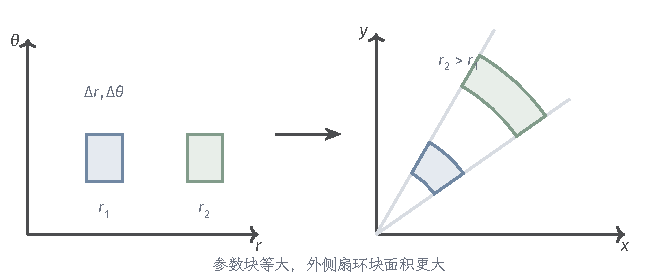
\includegraphics[width=112mm]{figures/00-shared/mathematical-preliminaries-upper/00-shared/tikz/mathematical-language-combinatorics-analysis-optimization-comprehension-additions/polar-area-weight.pdf}
\caption{径向宽度和角度宽度相同时，半径越大，对应的面积越大。小块的一阶面积为$r\Delta r\Delta\theta$，由此得到极坐标的面积权重。}
\label{fig:vol3-classical-polar-weight}
\end{figure}

极坐标在闭参数矩形上不满足换元定理的条件：原点处行列式为零，角度的两端又表示同一条射线。处理办法是先截断。限制$r\geq\varepsilon$且$\varepsilon\leq\theta\leq2\pi-\varepsilon$，在这个紧区域上应用换元定理，再令$\varepsilon\downarrow0$。
对于圆盘上的连续函数，去掉的小圆盘和窄扇形的贡献不超过函数的上界乘它们的面积，趋于零；参数一侧遗漏的部分也由有界的权重控制。

例如半径为$R$的圆盘面积为
\[
 \int_0^{2\pi}\int_0^R r\,\mathrm dr\,\mathrm d\theta=\pi R^2.
\]
若角度取到$4\pi$，圆盘内部被覆盖两次，结果也变成两倍。被积函数有奇点时，不能只说“接缝不贡献面积”而跳过截断的极限估计。

柱坐标在极坐标之外保留高度$z$，体积权重仍含因子$r$：
\[
 \mathrm dV=r\,\mathrm dr\,\mathrm d\theta\,\mathrm dz.
\]
由此，半径为$R$、高为$H$的圆柱体积为$\pi R^2H$。轴线和角度接缝的处理与极坐标相同。

球坐标使用到原点的距离$\rho$、从正$z$轴量起的极角$\varphi$和方位角$\theta$：
\[
 T(\rho,\varphi,\theta)
 =(\rho\sin\varphi\cos\theta,\rho\sin\varphi\sin\theta,\rho\cos\varphi).
\]
三个参数各自变化时，点沿三个相互正交的方向移动，长度的放大比例分别是$1$、$\rho$和$\rho\sin\varphi$。三者相乘就是体积权重，直接计算Jacobian行列式也得到同一结果：
\[
 \mathrm dV=\rho^2\sin\varphi\,\mathrm d\rho\,\mathrm d\varphi\,\mathrm d\theta.
\]

在$\rho>0$、$0<\varphi<\pi$和一个长度为$2\pi$的开角度区间上，这个映射是双射，像是空间去掉$z$轴和一个接缝半平面后的部分。计算球内连续函数的积分时，先截去原点、极轴和接缝附近的小区域，再用函数的有界性估计遗漏的部分。由此得到球的体积
\[
 \int_0^{2\pi}\int_0^\pi\int_0^R
 \rho^2\sin\varphi\,\mathrm d\rho\,\mathrm d\varphi\,\mathrm d\theta
 =\frac{4\pi R^3}{3}.
\]

\subsection{线性换元}

线性换元可以把斜着放的区域变成坐标盒。
设$D$由$0\leq x+y\leq2$和$0\leq x-y\leq2$围成，求$\int_D(x+y)\,\mathrm d(x,y)$。令$u=x+y$、$v=x-y$，参数区域就是$[0,2]^2$，逆变换为
\[
 x=\frac{u+v}2,\qquad y=\frac{u-v}2.
\]
逆变换的Jacobian行列式为$-1/2$，所以面积权重为$1/2$。于是
\[
 \int_D(x+y)\,\mathrm d(x,y)
 =\int_0^2\int_0^2\frac u2\,\mathrm du\,\mathrm dv=2.
\]

这个结果可以用另外两个量核对。取被积函数为$1$，同样的换元给出区域面积$2$。$x+y=u$在区域上的平均值为$1$，平均值乘面积也是$2$。区域、权重和积分值由此得到同时检验。

\section{参数积分}

若被积函数还依赖一个参数，积分值就随参数变化，成为参数的函数。例如一块薄板的密度随时间改变，总质量就是时间的函数。
判断这个函数是否连续、能否求导，需要控制整个积分区域上的变化；只在每一点处成立的极限不够。本节固定紧Jordan区域$D$，用连续性提供这种统一的控制。

\subsection{参数积分的连续性}

设$K$为紧参数区域，$f$在$D\times K$上连续，记
\[
 F(\bm t)=\int_D f(\bm x,\bm t)\,\mathrm d\bm x.
\]
$D\times K$是紧集，$f$在其上一致连续，所以$\bm t\to\bm s$时，
\[
 \sup_{\bm x\in D}|f(\bm x,\bm t)-f(\bm x,\bm s)|\longrightarrow0.
\]
用绝对值估计，
\[
 |F(\bm t)-F(\bm s)|
 \leq |D|\sup_{\bm x\in D}|f(\bm x,\bm t)-f(\bm x,\bm s)|\longrightarrow0,
\]
所以$F$连续。
参数区域不必整体有界。讨论某个内点附近的连续性时，取包含该点的一个小闭盒作为$K$即可。

\subsection{积分号下求导}

求导的思路相同：把参数差商的极限放进积分号内，关键是证明差商对所有$\bm x\in D$一致收敛。

设参数取自开集，$f$和各参数偏导数$\partial_{t_j}f$在$D$与参数邻域的乘积上连续。固定一个参数点，取它的一个足够小的闭邻域。由一元中值定理，沿$t_j$方向的差商等于附近某个参数处的偏导数值。偏导数在紧集上一致连续，所以差商对全部$\bm x\in D$一致趋于$\partial_{t_j}f$。对差商与偏导数之差积分，并用上一小节的上确界估计，得到
\begin{equation}
 \partial_{t_j}F(\bm t)=\int_D\partial_{t_j}f(\bm x,\bm t)\,\mathrm d\bm x.
\label{eq:classical-differentiate-under-integral}
\end{equation}

右侧又是一个被积函数连续的参数积分，由上一小节，它是参数的连续函数。于是$F$的各个偏导数都存在且连续，由连续偏导数判据，$F$是$C^1$函数，全微分为
\[
 DF_{\bm t}[\bm h]=\int_D D_{\bm t}f(\bm x,\bm t)[\bm h]\,\mathrm d\bm x.
\]
整体可微是由连续偏导数推出的；只验证每个方向上的极限，还不能得到这一结论。

例如$F(t)=\int_0^1 e^{tx}\,\mathrm dx$在任意有界参数区间上都满足上述条件，所以
\[
 F'(0)=\int_0^1x\,\mathrm dx=\frac12.
\]
显式表达式$F(t)=(e^t-1)/t$在$t=0$处有可去奇点；在积分号下求导，就不必处理它。

\subsection{变限参数积分}

积分区间也随参数变化时，积分值的变化来自两部分：区间内部的被积函数在变，两端又新添或移除了细条。

设$a(t),b(t)$为$C^1$函数，$f(x,t)$及$\partial_tf(x,t)$在所需区间附近连续。把积分写成从某个固定点到$b(t)$的积分减去从该点到$a(t)$的积分，对上限用一元基本定理，对被积函数中的参数用式~\eqref{eq:classical-differentiate-under-integral}，再由链式法则合并，得到
\begin{equation}
 \frac{\mathrm d}{\mathrm dt}\int_{a(t)}^{b(t)}f(x,t)\,\mathrm dx
 =\int_{a(t)}^{b(t)}\partial_tf(x,t)\,\mathrm dx
 +f(b(t),t)b'(t)-f(a(t),t)a'(t).
\label{eq:classical-variable-limit-derivative}
\end{equation}
第一项来自被积函数的变化，后两项来自端点的移动。上端向右移动会增加积分，下端向右移动会减少积分，所以两个边界项符号相反。

有多个参数时，对每个参数分别求偏导；也可以把$a'$、$b'$和$\partial_tf$换成作用于同一参数增量的全微分。更一般的移动区域会产生沿整个边界的贡献，本章只在上述区间变限的情形使用这一规则。

\FloatBarrier
\section{本章小结}
\label{sec:region-integrals-summary}

区域积分把密度累计成总量。Jordan区域是能用有限个坐标盒从内外两侧任意逼近的有界集合，等价地，它的边界能被总体积任意小的有限个盒覆盖。边界因而不影响有界函数的累计：在区域闭包上连续的函数可积，分块连续的有界函数也可积；有界本身则不够，例如有理点的指示函数不可积。积分继承有限和的线性、保序、绝对值估计与区域可加性，体积、质量、平均值和质心都是区域积分。

累次积分把一次多维累计化为几次一元积分。被积函数连续、区域由连续的边界函数描述时，按截面分组的Riemann和收敛到累次积分，两种次序给出同一个值；换序时要重新求出区域在另一坐标轴上的投影和截面，必要时改变分块。区域无界或被积函数无界时，有界情形的结论不能直接使用：要先截断再取极限，而不同的截断方式和不同的积分次序可以给出不同的结果。

换元时，可微映射在一点附近近似线性，Jacobian行列式的绝对值给出局部体积的缩放，换元公式把这些倍数累计起来。公式要求两个开集之间的$C^1$双射及$C^1$逆，绝对值消去的是定向的符号，消不去覆盖次数。极坐标、柱坐标和球坐标的权重分别为$r$、$r$与$\rho^2\sin\varphi$；它们在原点、轴线和角度接缝处不满足条件，须先截去这些部分，再用被积函数的有界性控制遗漏的贡献。

参数积分在紧Jordan区域上依赖统一控制：被积函数在区域与参数集的乘积上连续时，积分随参数连续；参数偏导数也联合连续时，可以在积分号下求导，并由连续偏导数推出全微分。只有逐点的极限不够。积分限随参数移动时，导数除了积分号下的项，还要加上两端新增或移除的细条贡献。下一章把累计的范围从区域换成曲线。

